\newpage
\section{Problem}

The goal of this project is to create a user-friendly application that can generate modern 3D cities, and then export them as \textit{.fbx} files.
\textit{User-friendly} means that users should need no technical expertise or coding experince to fully utilize the application.
\textit{Modern cities} means that the cities should resemble modern industrialized
cities such as New York, Paris, San Francisco, and Tokyo. Figure \ref{fig:ModernCities}
showcases two examples of such modern cities.

\begin{figure}[h!]
  \centering

  \begin{subfigure}[b]{0.48\textwidth}
    \frame{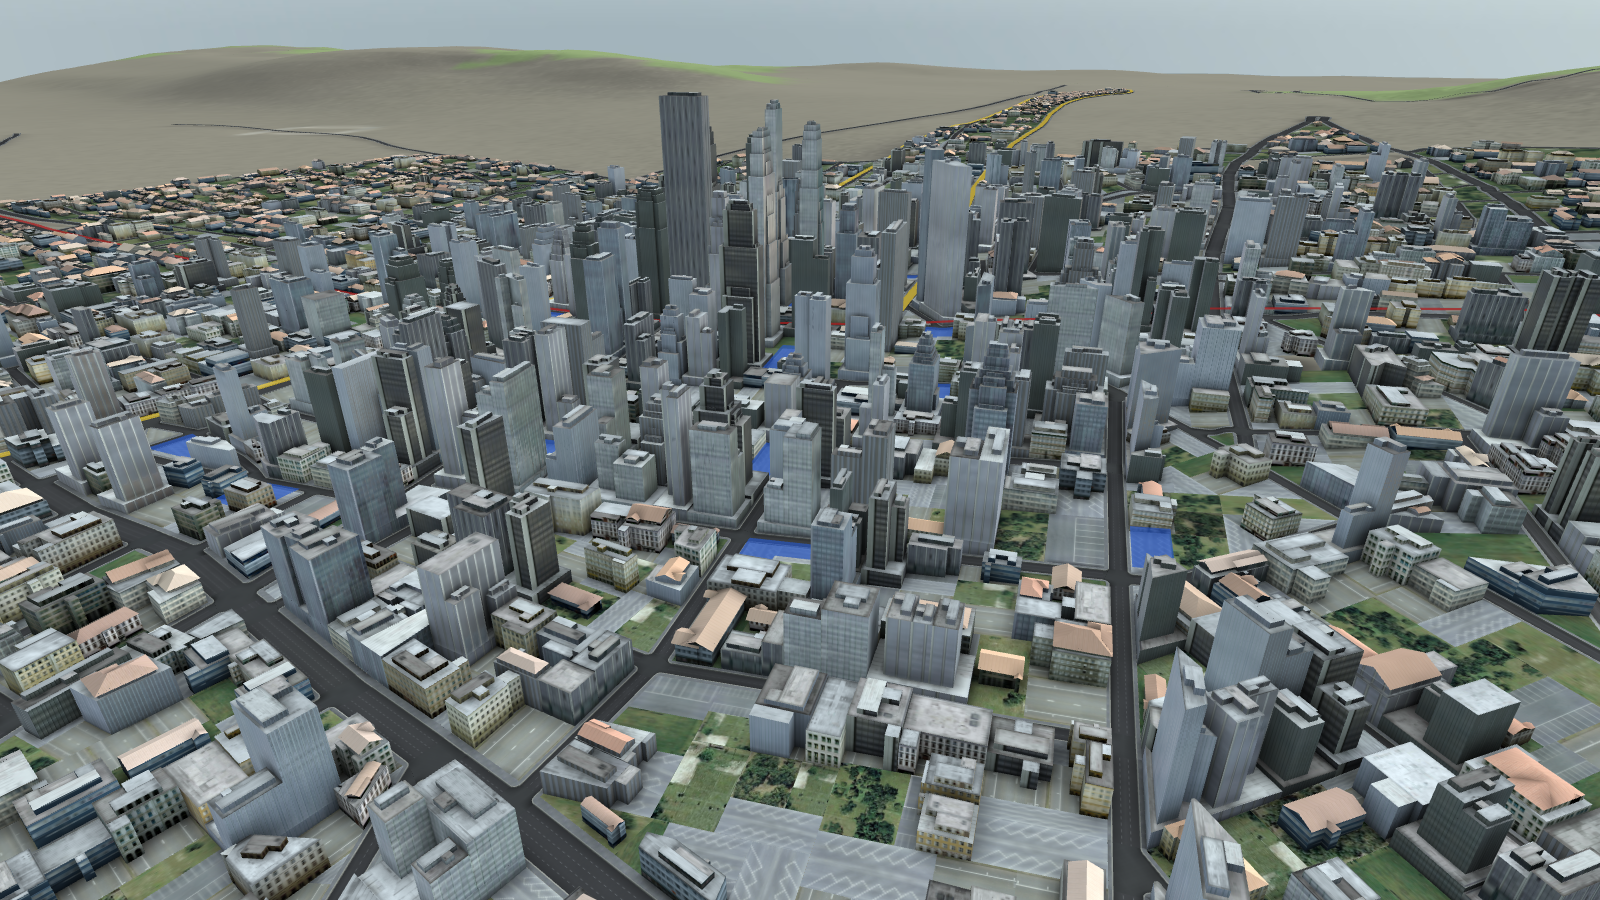
\includegraphics[width=\textwidth]{figure/modern-city.png}}
  \end{subfigure}
  \quad
  \begin{subfigure}[b]{0.48\textwidth}
    \frame{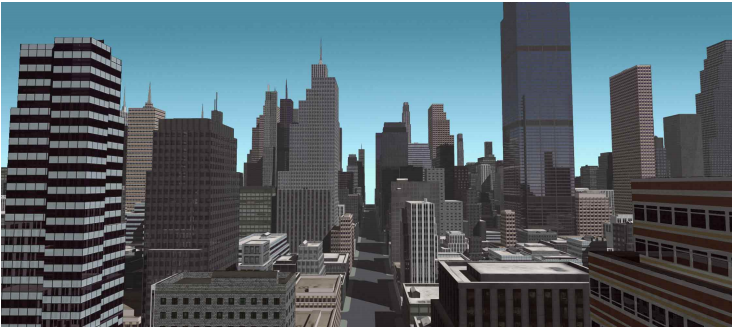
\includegraphics[width=\textwidth]{figure/modern-city2.png}}
  \end{subfigure}

  \caption{Examples of generated modern cities from related works \cite{yoav_and_pascal}\cite{cl3ver}.}
  \label{fig:ModernCities}
\end{figure}

It is worth clarifying that suburban areas and rural areas are also included as
part of such cities.

The focus will be put on the roads and the buildings of the city, and not on the
terrain around it. The surrounding terrain should help create interesting scenarios for the cities to adjust to.

The user will interact with the program in the following way:
\begin{enumerate}
  \item The user specifies the size of the world in terms of a 2D plane.
  \item The user specifies any optional parameters that affect the terrain
    such as sea level.
  \item The user clicks on a button that says ``Generate Terrain'' as many times
    as they like, until they are satisfied with the generated terrain.
  \item The user then selects which region of the generated terrain they want to use in the final model.
  \item The user places population markers on the terrain and specifies how much
    population each marker represents. The user can also specify any optional
    parameters for each city such as road type.
  \item The user clicks on a button that says ``Generate Roads'' as many times
    as they like, until they are satisfied with the generated road network.
  \item The user clicks on a button that says ``Generate Buildings'' as many times
    as they like, until they are satisfied with the generated buildings.
  \item Finally, when the user is satisfied with the result they can click on a
    button that says ``Export to FBX'' and the the program will save the full
    model as a \textit{.fbx} on the local filesystem.
\end{enumerate}
These interactions should occur through a user-friendly Graphical User Interface
(GUI).

The problem can be divided into 3 major subproblems: generation of landscape, road networks, and buildings.
Each of the following subsections will go into more detail about these subproblems.

\subsection{Terrain Generation}

e.g. steep hills, rivers, and ocean.
To start with, the algorithm has to create terrain, roads, cells and entities. 

The user will provide a value for the sea level in the form of a number, and we will color the terrain based on the height levels e.g. grasslands near sea level, rocky mountain textures for the taller regions, and snow for top peaks of some of the taller mountains.

\subsection{Road Generation}
\subsection{Building Generation}
